\documentclass[../PFC.tex]{subfiles}
\begin{document}

\section{Seguridad}
\label{Seguridad}

Existen ciertas consideraciones básicas a tener en cuenta respecto a la seguridad de la identificación y comunicaciones. Siempre ha sido un elemento primordial el poder identificar el emisor de un mensaje y el contenido no haya sido manipulado. 
\\\\
Existen claros ejemplos de que es un problema al cuál se le han puesto diversas soluciones a lo largo de los siglos en diferentes civilizaciones. Las comunicaciones han sido desde hace milenios un elemento esencial para diferentes objetivos, pese a que, en la mayoría de los casos, la aplicación inicial ha sido bélica. Ganar ventaja sobre un enemigo en cualquier ámbito podría significar la diferencia entre la victoria o la consecución del objetivo o no. La seguridad en las comunicaciones no se encuentra exenta de ello. 
\\\\
El ejemplo más evidente y referenciado en numerosos filmes es el del envío de un mensaje sellado con la marca identificadora del emisor. Esta práctica es conocida hace más de 3.000 años para firmar documentos oficiales por parte de mandatarios. Se habla más en profundidad en el libro de Randall Price: \textit{The stones cry out}\cite{stonesCryOut} sobre las investigaciones y descubrimientos, entre ellos las del arqueólogo Avraham Biran, que corroboran la afirmación de la utilización de sellos identificativos por parte del reinado del rey David en Israel (dicha identificación hace prueba de su existencia, tema controvertido). Básicamente se realizó el mismo procedimiento durante cientos de años: escribir una misiva con contenido sensible, sellar la misiva con una cuña identificativa y entregar el mensaje al destinatario. El sello se presuponía único ya que dicha cuña solo se encontraba en posesión de un emisor válido. Al sellarse, se aseguraba la integridad de que el contenido no fuera comprometido si no se rompía el sello. El receptor obtenía la carta con el sello y el mensaje original en su interior, siendo capaz de responder de una forma idéntica si se diera el caso.
\\\\
Este sistema no era perfecto, pero conseguía grandes resultados en su época ya que la copia de un sello no era tan sencilla como se podría imaginar. Sin embargo, los inconvenientes de su utilización resultan obvios: mensajes entregados erróneamente o capturados durante su trayecto, desconocimiento de la validez del sello, aperturas de la carta por otros medios, tiempo de entrega, validez temporal del mensaje y etcétera.
\\\\
Con el paso del tiempo cambiaron los canales de comunicación. Los sistemas de comunicaciones dieron pasos de gigante con inventos tales como la telegrafía óptica (emitir mensajes en la distancia mediante la disposición de elementos visibles en diferentes posiciones), la invención del teléfono por parte de Antonio Meucci o el telégrafo por parte de S. Morse. Con ello aumentaron la capacidad, rapidez y la eficacia de las comunicaciones, pese a que por otro lado se producían nuevos problemas de identificación.
\\\\
Actualmente, hasta las comunicaciones más simples cuentan con sistemas que aseguran que la identidad de las partes implicadas sean veraces y el contenido seguro. No por ello dejan de existir partes malintencionadas que buscan obtener información o adulterarla en base a sus pretensiones; para evitarlo nace la criptografía. La criptografía había sido estudiada (criptología) desde hace siglos, donde va cobrando vital importancia desde sus inicios debido a las aplicaciones para realizar comunicaciones seguras.

\section{Criptografía}
\label{Criptografía}

La criptografía (del griego \textit{cripto} (oculto) y \textit{logo} (grafo) o escritura oculta) actualmente 'se encarga del estudio de los algoritmos, protocolos y sistemas que se utilizan para dotar de seguridad a las comunicaciones, a la información y a las entidades que se comunican'\cite{pastor1998criptografia}. La implementación de criptosistemas (sistemas criptográficos) ha sido utilizada desde las más básicas trasposiciones de caracteres de la época romana hasta los más avanzados de la actualidad con la utilización de propiedades matemáticas avanzadas.
\\\\
Dentro de los métodos más básicos se encuentran aquellos referidos a la criptografía clásica. Ésta utilizaba en su mayoría la trasposición como elemento de cifrado y descifrado. El algoritmo César, utilizado por Julio César para enviar mensajes secretos\cite{lucena}, constaba únicamente de transformar las letras del mensaje por la letra 3 posiciones a la derecha respecto a su número de orden en un diccionario. Así, la letra $A$ se transforma por la $D$, la $B$ por la $E$, y así sucesivamente. Contando con un diccionario de 26 letras su definición vendría dada por $C= (M + 3)\  mod\ 26$. El mensaje cifrado final $M$ es la composición de los diferentes caracteres del mensaje $M$ transformados en $C$.
\\\\
En algunos sistemas UNIX se encuentra otro ejemplo de criptografía clásica como lo es ROT13. En el fondo no tiene intenciones criptográficas. Sin embargo, sirve de ejemplo práctico de la idea de cómo se usaba la criptografía en sus inicios. ROT13 es análogo al algoritmo César, en vez de desplazar tres letras al caracter $M$ del mensaje original se desplazan trece. Con ésto se consigue realizar un ciclo si se aplica el procedimiento dos veces; la propia función de encriptación es la desencriptación. Así pues, encriptando un mensaje $P$ dos veces con ROT13 se obtiene el mensaje original : $P = ROT13 (ROT13 (P))$.
\\\\
Durante la segunda guerra mundial cobró gran relevancia la criptografía utilizada por el bando alemán para sus comunicaciones. La máquina que se utilizaban es la conocida \textit{ENIGMA}. Inventado por Arthur Scherbius y Arvid Gerhard Damm\cite{bruce}, basaba su comportamiento en la posición de tres rotores a la hora de escribir con dicha máquina. La posición de los rotores se podía modificar y la fuerza del sistema residía en que la posición de dichos rotores era secreta. La seguridad en este sistema se vio comprometida en varias ocasiones durante la guerra ya que, aunque no era trivial, había que averiguar únicamente la combinación de los rotores. Para evitarlo, el bando alemán cambia la posición de los rotores a una nueva versión aunque fuera eventualmente descifrado por el bando enemigo.
\\\\
Con este último ejemplo vemos la fragilidad de un sistema criptográfico si existe una relación directa entre el mensaje cifrado y el descifrado. El matemático Claude Elwood Shannon definió un modelo matemático qué describía lo que significa ser seguro para un criptosistema\cite{bruce}. En este modelo habla sobre la importancia de que la información que brinda un mensaje cifrado no debería aportar nada sobre el mensaje cifrado, esto sería un sistema perfecto. Los mejores criptoanálisis se nutren de esta información que ofrece el mensaje cifrado; por lo que los buenos algoritmos criptográficos buscan que la información que los relaciona sea mínima. Los criptoanalistas aprovechan la redundancia del lenguaje natural para efectuar técnicas como el análisis de frecuencias. Así, también es común utilizar la eliminación de la redundancia antes de encriptar los mensajes.
\\\\
Otra forma de saber como de seguro es un algoritmo criptográfico es el nivel de entropía (o entropía de Shannon). La entropía refleja la incertidumbre de una fuente de información. Shannon define su entropía como máxima si todos los sucesos son equiprobables \cite{shannon2001mathematical}, si esto se da en un sistema criptográfico significa que formándose cierta codificación no hay información que ayude a saber cuál la sigue. También es importante la clave utilizada y el tamaño y lenguaje que se obtiene al encriptar, contra mayor sea la variedad y el tamaño mínimo generado en un mensaje cifrado, más difícil computacionalmente será calcular el mensaje original. Uniendo la información que brinda un mensaje cifrado sobre el mensaje original junto a una entropía máxima obtenemos un criptosistema seguro; 'esto significa sencillamente que la distribución de probabilidad que nos inducen todos los posibles mensajes en claro cambia si conocemos el mensaje cifrado'\cite{lucena}.
\\\\
Un criptosistema se define como una quintupla $(M,C,K,E,D)$ descrita a continuación\cite{lucena}:

\begin{itemize}
\item{$M$ es el mensaje sin cifrar.}
\item{$C$ es el mensaje cifrado.}
\item{$K$ es el conjunto de claves que emplea el criptosistema.}
\item{$E$ es la función que utilizando $K$ transforma el mensaje $M$ en $C$.}
\item{$D$ análogo a $E$ es el conjunto de transformaciones de descifrado.}
\end{itemize}

Existen dos tipos de criptosistemas: simétricos y asimétricos. Todo criptosistema simétrico debe cumplir que con un mensaje cifrado $C$ se desencripta utilizando la misma clave $k$ empleada a la hora de encriptar el mensaje original $M$:

\begin{center}
\begin{equation}
D_{k}(E_{k}(m)) = m
\end{equation}
\end{center}

Por el contrario, un criptositema asimétrico emplea una clave pública $p$ y otra privada $k$ para encriptar y desencriptar respectivamente:

\begin{center}
\begin{equation}
D_{k}(E_{p}(m)) = m
\end{equation}
\end{center}

A continuación se muestran ciertos protocolos de ambos tipos de criptosistemas.

\subsection{Protocolos simétricos y asimétricos}
\label{Protocolos simétricos y asimétricos}

Para que las comunicaciones sean seguras se utiliza encriptación. Por lo que es necesario ponerse de acuerdo en la forma de comunicarse. Para la comunicación basada en criptografía simétrica se describe el siguiente protocolo base dado el ejemplo si Alice quisiera enviarle un mensaje a Bob\cite{bruce}:

\begin{itemize}
\item[1]{Alice y Bob se ponen de acuerdo en un criptosistema simétrico.}
\item[2]{Alice y Bob se ponen de acuerdo en una clave de cifrado $k$.}
\item[3]{Alice encripta el mensaje usando el algoritmo de encriptación del criptosistema y la clave acordada. Se genera un mensaje cifrado.}
\item[4]{Alice envía el mensaje cifrado a Bob.}
\item[5]{Bob desencripta el mensaje cifrado con el algoritmo de desencriptación y la clave y obtiene el mensaje original.}
\end{itemize}

Existiendo un tercer personaje en este ejemplo, Eve, podría intentar entrometerse en la comunicación. Si Eve escuchara el paso 4 del protocolo obtendría el mensaje cifrado. Con ello podría intentar efectuar criptoanálisis y obtener el texto original. Sin embargo, existen algoritmos bastante seguros para evitar exponer la información pese a ataques de este tipo.
\\\\
No obstante, Eve sabe que el objetivo en este protocolo sería interponerse en la comunicación para escuchar los puntos 1 y 2. Así, cuando se alcanzara el paso 4 solo tendría que realizar la misma operación que haría Bob para recuperar el mensaje original. Un buen criptosistema debería relegar la seguridad del criptosistema al conocimiento de la clave y no al del algoritmo que se emplea. Por ello, realizar el paso 1 en público no debería ser un problema, sin embargo, el paso 2 para elegir la clave debería ser secreto entre Alice y Bob. Con ello se reutiliza la clave para encriptar y desencriptar. Por otra parte, además de que la clave está comprometida si no se distribuye en secreto, los protocolos simétricos disponen de un problema con el tamaño de las claves: hay una clave disponible para cada comunicación entre los usuarios. Por ejemplo, un sistema de 10 usuarios necesitaría 45 claves válidas distintas ( necesitando $n(n-1)/2$ claves para $n$ usuarios).
Los protocolos asimétricos buscan solucionar este problema otra forma.
\\\\
Los protocolos asimétricos o de clave pública disponen de una clave pública por usuario, disponible a todo el mundo, y una clave privada personal que no se comparte con nadie. En este protocolo, Alice posee una clave pública que es conocida por Bob y otra clave privada que no es conocida por nadie más que Alice y viceversa. Por lo que las acciones quedarían de la siguiente forma :

\begin{itemize}
\item[1]{Alice y Bob se ponen de acuerdo en un criptosistema de clave pública.}
\item[2]{Alice consulta la clave pública de Bob $k$.}
\item[3]{Alice encripta el mensaje usando el algoritmo de encriptación del criptosistema y la clave privada de Bob. Se genera un mensaje cifrado.}
\item[4]{Alice envía el mensaje cifrado a Bob.}
\item[5]{Bob desencripta el mensaje cifrado con el algoritmo de desencriptación y la clave privada y obtiene el mensaje original.}
\end{itemize}

Ahora Eve no es capaz de desencriptar el mensaje ya que para ello necesita la clave privada de Bob. Las claves públicas de cada uno de los usuarios se pueden disponer en cualquier lugar de acceso público. Lo único que puede hacer es encriptar un mensaje con la clave pública de un usuario y éste será el único que pueda desencriptarlo. El problema que tiene este tipo de sistemas es la distribución de claves, que ha de ser privado.
\\\\
También existen sistemas híbridos que utilizan un protocolo asimétrico para acordar una clave y luego utilizar ésta para realizar la encriptación y desencriptación como se haría en un protocolo simétrico. Nuevamente, la idea principal es salvaguardar la clave utilizada para desencriptar el mensaje, para ello, los criptosistemas utilizan algoritmos basados en propiedades matemáticas que aseguran una complejidad muy elevada (teóricamente imposible) para obtener dicha clave. El problema del logaritmo discreto es un ejemplo de propiedades matemáticas que utilizadas en los criptosistemas más seguros.

\subsection{Problema del logaritmo discreto}
\label{Problema del logaritmo discreto}

Muchos de los criptosistemas utilizan exponenciaciones con magnitudes enormes. Tanto la base como el exponente pueden ser de cientos de bits de longitud y usualmente primos para evitar la factorización. Así pues, el calculo del valor resultante de esas exponenciaciones requiere de algoritmos eficientes. 
\\\\
Por otro lado, la operación inversa a la exponenciación es el cálculo de logaritmos discretos. Dados dos números $a$, $b$ y el módulo $n$, se define el logaritmo discreto de $a$ en base $b$ módulo n como\cite{lucena}:

\begin{equation}
c = log_{b}(a)\ (mod\ n)\ \Leftrightarrow a \equiv b^c\ (mod\ n)
\end{equation}

No existen algoritmos eficientes que computen estos logaritmos de estas características en tiempo razonable, lo cuál hace que sea una propiedad base para la robustez del sistema de numerosos sistemas criptográficos.


\subsection{Criptología con curvas elípticas - ECC}
\label{Criptología con curvas elípticas - ECC}

\textit{Definición}: Una curva elíptica sobre los números reales $\mathbb{R}$ es el conjunto de puntos del plano $(x , y)$ que cumplen la siguiente ecuación\cite{bruce}:

\begin{equation}
y^2 = x^3 + ax + b
\end{equation}

Con los puntos de la curva dados por la ecuación anterior (evitando singularidades con los valores $a = 4$ y $b = 27$), junto a un punto en el infinito $O$ y la operación de suma se denomina grupo de curva elíptica $E(\mathbb{R})$. La visualización gráfica de una curva elíptica es la mostrada en la figura \ref{img:ec}

\begin{figure}[H]
  \centering
  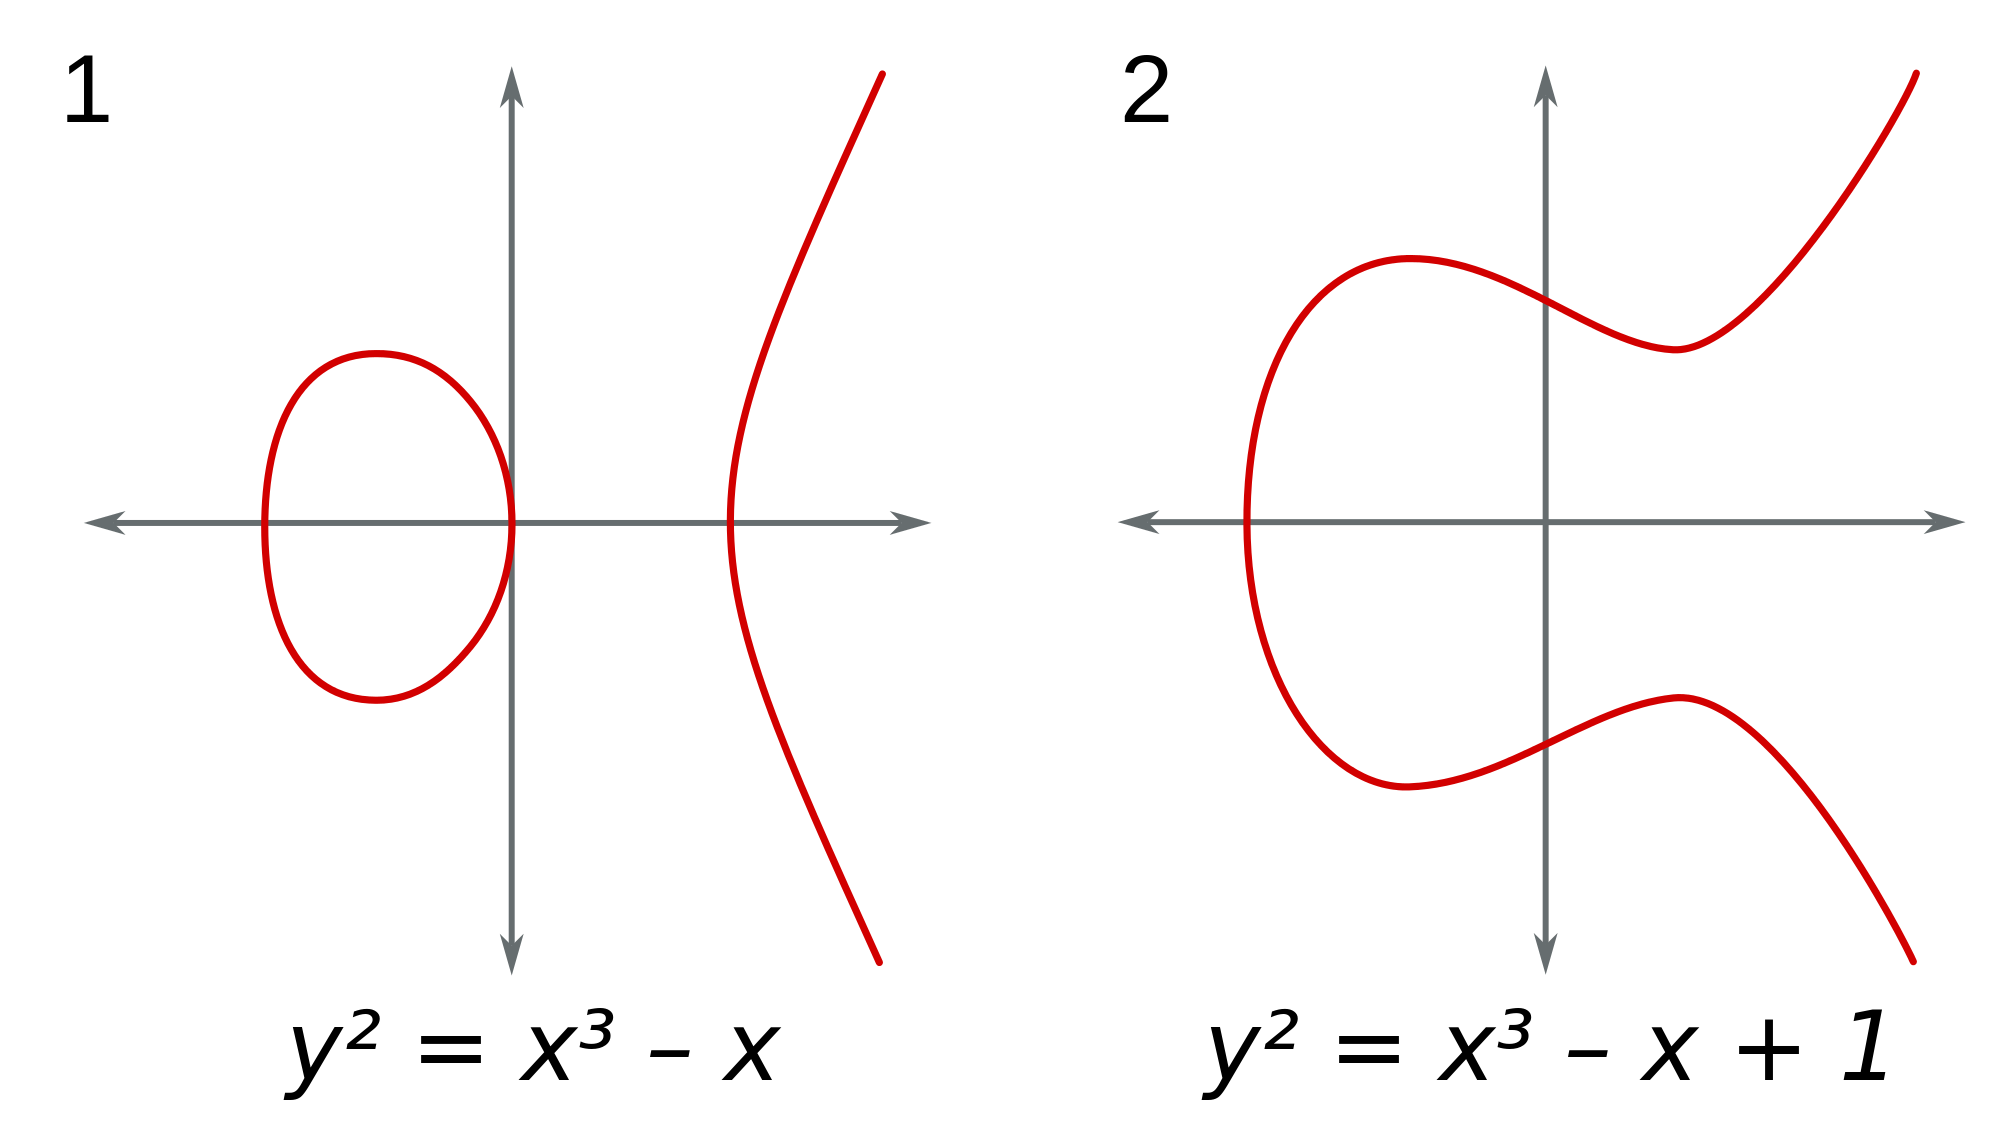
\includegraphics[width=0.7\textwidth]{./img/EC}
  \caption{Visualización de las curvas elípticas más representativas.}
  \label{img:ec}
\end{figure}

Un cuerpo finito de \textit{Galois} $GF(n)$ es un grupo finito generado por $n$, siendo $n$ primo \cite{lucena}. Por lo que se define $E(GF(2^n))$ como los puntos dentro de un grupo finito dados por una curva elíptica generados por un número en base 2 exponenciado por otro número primo alto. Por lo que se forman pares de polinomios de grado $n-1$ con coeficientes binarios, fácilmente representables por cadenas de bits\cite{lucena}.

\begin{equation}
y^2 + xy = x^3 + ax^2 + b\ (mod 2^n)
\end{equation}

No vamos a entrar en detalle cómo es la suma de puntos en una curva elíptica. Pero podemos observar visualmente cómo se realizan estas operaciones con puntos $P$,$Q$ y el uso del punto en el infinito $O$ en la figura \ref{img:ecc}. En la figura se muestra cómo se calcula la recta que une los puntos a sumar, el uso de la tangente para sumas con el mismo punto y sus relaciones con el punto en el infinito.

\begin{figure}[H]
  \centering
  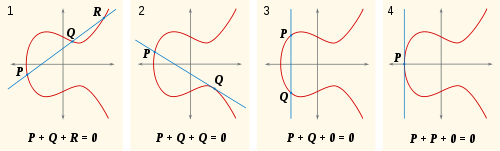
\includegraphics[width=1\textwidth]{./img/ECC}
  \caption{Suma de puntos en una curva elíptica.}
  \label{img:ecc}
\end{figure}

Si disponemos de un punto $q$ perteneciente a un conjunto de la suma de un punto $p$ tantas veces como permita el campo finito definido, debe existir un número entero $k$ tal que $kp = q$. 'El Problema de los logaritmos discretos en curvas elípticas consiste precisamente en hallar el número $k$ a partir de $p$ y $q$. Hasta ahora no se ha encontrado ningún algoritmo eficiente (subexponencial) para calcular el valor de $k$. Este problema puede ser empleado con éxito para el desarrollo de algoritmos criptográficos de llave pública.'\cite{lucena}.
\\\\
El uso de criptosistemas con curvas elípticas emplea claves de un tamaño reducido respecto a otros sistemas de encriptación asimétricos considerados seguros. A su vez, para tener un sistema seguro durante todo el siglo XIX y con una evolución de la tecnología siguiendo la ley de Moore triple (cada año la capacidad computacional aumenta el triple), se recomienda utilizar sistemas simétricos de 135\textit{bits} de tamaño de claves y asimétricos de 1550\textit{bits} (siguiendo las teorias del matemático Arjen K. Lenstra en su documento\cite{lenstra}). Sin embargo, para curvas elípticas recomiendan tamaños de claves de 270 \textit{bits}. La ventaja de la criptografía de las curvas elípticas es considerable evitando utilizar únicamente un sistema simétrico\cite{keylength}.
\\\\
Más en profundidad, los autores Steven D. Galbraith y Pierrick Gaudry elaboraron el documento \cite{galbraith2016recent} en el cuál estudian los problemas computacionales relacionados con el problema del logaritmo discreto y su relación con las curvas elípticas. A su vez, también comentan ataques de criptoanálisis para diferentes definiciones de curvas elípticas (paso de gigante paso de niño o el algoritmo \textit{lambda} de Pollard entre otros).

\section{Tecnología NFC}
\label{Tecnología NFC}

La tecnología NFC o \textit{Near Field Communication} es un sistema de comunicación entre dispositivos basado en radiofrecuencia, que deriva de la tecnología \textit{RFID} (\textit{Radio Frequency IDentification}), definido en el estándar ISO-14443\cite{iso14443}. El chip NFC contiene la capacidad de información limitada del orden de 64 \textit{bytes} a los 4\textit{Kb} de los chips NFC \textit{MIFARE Classic 4k}.
\\\\
La lectura del contenido se realiza mediante la inducción de un campo magnético del dispositivo de lectura al chip contenedor de la información. Funciona en la banda de frecuencia 13.56\textit{Mhz} por lo que no está vinculado a ninguna normativa de uso ni restricción. Estos chips ha conquistado numerosos ámbitos debido a la utilidad que proveen a la hora de comunicar información con costes muy reducidos y elementos fácilmente transportables.

\end{document}